%%%%%%%%%%%%%%%%%%%%%%%%%%%%%%%%%%%%%%%%%%%%%%%%%%%%%%%%%%%%%%%%%%%%%%%%
% vim:enc=utf-8:ts=5:sw=5:et:ff=unix:
%%%%%%%%%%%%%%%%%%%%%%%%%%%%%%%%%%%%%%%%%%%%%%%%%%%%%%%%%%%%%%%%%%%%%%%%

\chapter{Introdução}
%
A edição de texto é uma das tarefas mais frequentemente executadas por seres
humanos em ambientes computacionais, em qualquer nível. Usuários finais,
administradores de sistemas, programadores de software, desenvolvedores {\em
web}, e tantas outras categorias, todos eles, constantemente, necessitam
editar textos. 

Usuários finais editam texto para criar documentos, enviar e-mails, atualizar
o blog, escrever recados ou simplesmente trocar mensagens instantâneas pela
internet. Administradores de sistemas editam arquivos de configuração, criam
regras de segurança, editam {\em scripts} e manipulam saídas de comandos
armazenados em arquivos de texto. Programadores desenvolvem códigos-fonte e a
documentação de programas essencialmente em editores de texto.  Desenvolvedores {\em web}
interagem com editores de texto para criarem {\em layout} e dinâmica de sites.

Tamanha é a frequência e onipresença da tarefa de edição de texto que a
eficiência, flexibilidade e o repertório de ferramentas de editores de texto
tornam-se quesitos críticos para se atingir {\em produtividade} e {\em
conforto} na edição de textos.
%
% falar da não trivialidade do aprendizado (curva de aprendizado), mas também
% da eficiência e produtividade a médio/longo prazo

O ``\href{http://www.vim.org}{Vim}''\footnote{Vim - \url{http://www.vim.org}}
\index{vim} é um editor de texto extremamente configurável, criado para permitir a
edição de forma eficiente, tornando-a produtiva e confortável. 
Também é uma aprimoração do editor ``Vi'', um tradicional programa dos
sistemas Unix. Possui uma série de mudanças em relação a este último. O
próprio slogan do Vim é {\em Vi IMproved}, ou seja, {\em Vi Melhorado}.  O Vim
é tão conhecido e respeitado entre programadores, e tão útil para programação,
que muitos o consideram uma verdadeira ``IDE\index{ide}\footnote{Ambiente Integrado de
Desenvolvimento.}''.

Ele é capaz de reconhecer mais de 500 sintaxes de linguagens de programação e
marcação, possui mapeamento para teclas, macros, abreviações, busca por
{\em{Expressões
Regulares}}\index{expressões regulares}\footnote{Expressões Regulares - 
\url{http://guia-er.sourceforge.net/guia-er.html}}, entre outras facilidades.

% NOTA: não estou convencido sobre a relevância desse conteúdo, fica pelo menos
% como um o primeiro exemplo.
% referenciando a figura. O til serve para evitar que o número fique 
% em um linha e o nome em outro.
% toda referência é feita antes de inserir a figura.
A figura~\ref{fig:vimedittex} mostra o vim sendo usando para editar o arquivo
o desse livro sobre vim.

% Inserindo apenas uma figura
% A opção [htp] é o melhor conjunto para livros, pois evita que a figura
% se afaste muito do texto onde é citado.
\begin{figure}[htp]
  % centralizando a figura
  \centering 
  % especficiando a figura
  % a figura não precisa ter extensão
  % width : define o tamanho lateral
  %         use a unidade que conhecer, px, m, mm, cm, in, etc.
  %         usar apenas essa opção assegura que a proporção seja mantida.
  %         é possível especificar a outra dimensão ou uma fator global, 
  %         exemplos estão comentados, para height (altura) e scale (escala)
  % tudo que está entre colchetes é opcional, e existem muitas opções para 
  % esse campo, mas o que está abaixo é suficiente em 90 % dos casos
  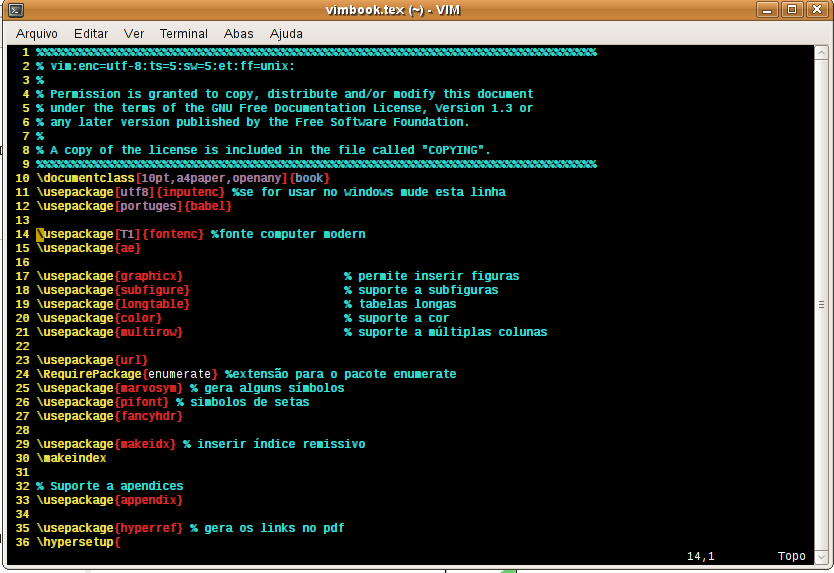
\includegraphics[width=9cm]{img/vimedittex} % 9 cm de lado
  %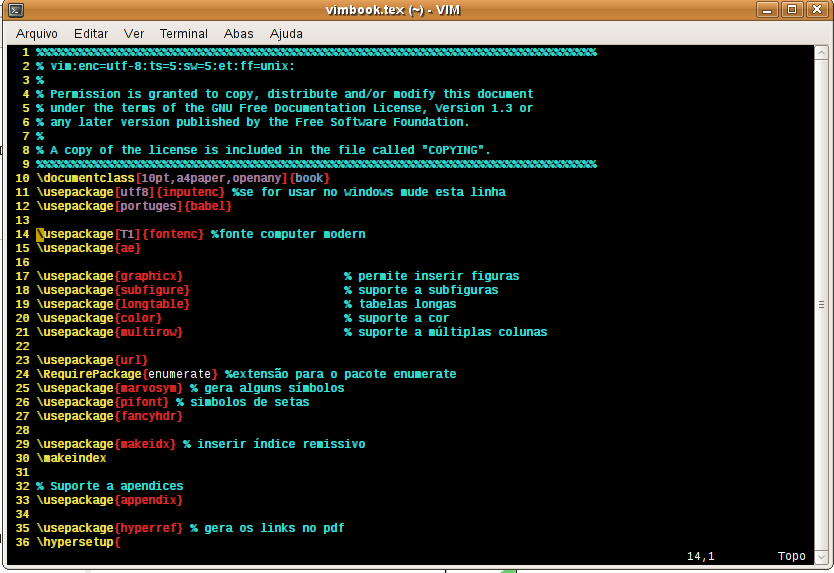
\includegraphics[height=7cm]{img/vimedittex} % 7 cm de altura
  %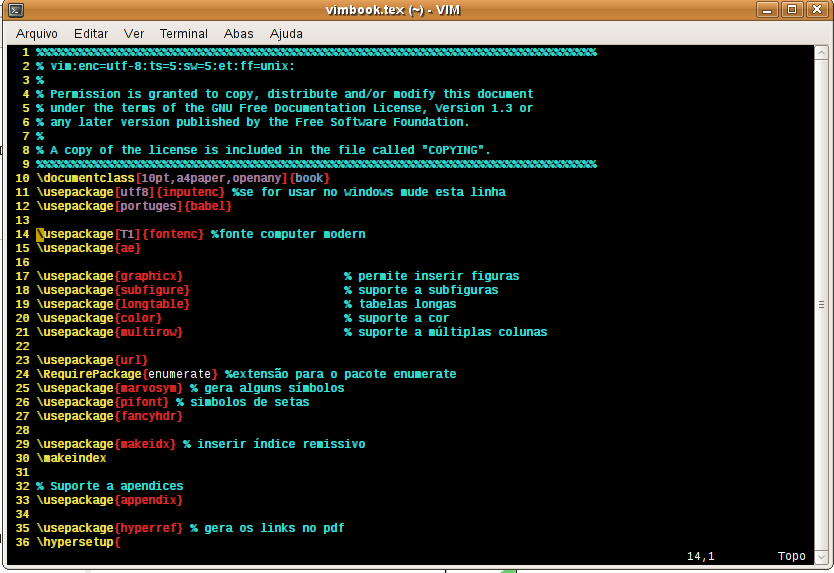
\includegraphics[scale=0.4]{img/vimedittex} % 40 % do tamanho real
  % legenda da figura, a legenda vem depois da figura.
  \caption{Usando o vim para editar o código em \LaTeX}
  % rotulado essa figura, é usando por \ref{} para citar a figura.
  \label{fig:vimedittex}
\end{figure}

O Vim conta com uma comunidade bastante atuante e é, ao lado do
Emacs\footnote{Emacs - \url{http://www.gnu.org/software/emacs/}}, um dos editores mais usados
nos sistemas GNU/Linux\footnote{O kernel Linux sem os programas GNU não
serviria para muita coisa.}, embora esteja também disponível em outros sistemas,
como o Windows e o Macintosh. %O site oficial do Vim é \url{http://www.vim.org}.

\section{Instalação do Vim}\index{vim!instalar}
\vimhelp{install}
%
\subsection{Instalação no Windows}
%
Há uma versão gráfica do Vim disponível para vários sistemas operacionais, incluindo o Windows;
esta versão pode ser encontrada no \href{http://www.vim.org/download.php#pc}{site
oficial}. 
Para instalá-lo basta baixar o instalador no link indicado e dispará-lo com um
duplo clique (este procedimento requer privilégios de administrador).

\subsection{Instalação no GNU/Linux}
%
A maioria das distribuições GNU/Linux traz o Vim em seus repositórios, sendo
que é bastante comum o Vim já vir incluído na instalação típica da distribuição.
A forma de instalação preferível depende do Vim:
\begin{itemize}
\item Já vir instalado por {\em default} -- neste caso nada precisa ser feito.

\item Estar disponível no repositório, mas não instalado -- em distribuições
derivadas da Debian GNU/Linux\footnote{Debian GNU/Linux - \url{http://www.debian.org/index.pt.html}},
a instalação do Vim através dos repositórios é usualmente executada
digitando-se {\tt `apt-get install vim'}\footnote{Recomenda-se também instalar
a documentação em HTML do Vim: {\tt `apt-get install vim-doc'}} em um {\em terminal} (este procedimento
requer privilégios de administrador e, tipicamente, conexão com a internet).

\item Não estar disponível no repositório da distribuição -- cenário {\em muito}
improvável, mas nas sua ocorrência o Vim pode ser instalado através da compilação do
código-fonte; basta seguir as instruções do \href{http://www.vim.org/download.php}{site oficial}.

\end{itemize}

\section{Dicas iniciais}\label{Dicas iniciais}
%
Ao longo do livro alguns comandos ou dicas podem estar duplicados, o que
é útil devido ao contexto e também porque o aprendizado por saturação
é um ótimo recurso. Ao perceber uma dica duplicada, antes de
reclamar veja se já sabe o que está sendo passado. Contudo dicas e sugestões serão bem vindas! 

Para abrir um arquivo\index{iniciar} com Vim digite num terminal:
%
\begin{verbatim}
     vim texto.txt
\end{verbatim}
onde {\tt texto.txt} é o nome do arquivo que deseja-se criar ou editar.

Em algumas distribuições, pode-se usar o comando {\tt vi} ao invés de {\tt vim}.

\section{Ajuda integrada}
%
O Vim possui uma ajuda\index{ajuda}\index{manual} integrada muito completa, são mais
de 100 arquivos somando milhares de linhas. O único inconveniente é não haver ainda
tradução para o português, sendo o inglês seu idioma oficial; entretanto, as explicações
costumam ser sintéticas e diretas, de forma que noções em inglês seriam
suficientes para a compreensão de grande parte do conteúdo da ajuda integrada.

Obs: No Vim quase todos os comandos podem ser abreviados, no caso
``\verb+help+'' pode ser chamado por ``\verb+h+'' e assim por diante. Um
comando só pode ser abreviado até o ponto em que este nome mais curto não
coincida com o nome de algum outro comando existente.  Para chamar a ajuda do
Vim pressione \verb|<Esc>| e em seguida:
%
\begin{verbatim}
     :help .... versão longa, ou
     :h ....... versão abreviada
\end{verbatim}
%
ou simplesmente:
%
\begin{verbatim}
     <F1>
\end{verbatim}

Siga os links usando o atalho ``\verb|Ctrl-]|'', em modo gráfico o clique com o
mouse também funciona, e para voltar use ``\verb|Ctrl-O|'' ou
``\verb|Ctrl-t|''. Para as situações de desespero pode-se digitar:

\begin{verbatim}
     :help!
\end{verbatim}

\section{Em caso de erros }\label{Em caso de erros }
%
Recarregue\index{em caso de erros} o arquivo que está sendo editado assim:

\begin{verbatim}
     <Esc> .. para sair do modo de edição
     :e! .... recarrega o arquivo sem qualquer edição
\end{verbatim} % quando se quer continuar um texto abaixo de uma região, 
               % não se pula linha para evitar parágrafo forçado
               % comentário não é pular linha
ou simplesmente inicie outro arquivo ignorando o atual, com
\begin{verbatim}
     :enew!
\end{verbatim}
%
ou saia do arquivo sem modifica-lo, com
%
\begin{verbatim}
     :q! .... saída forçada, nada é alterado
\end{verbatim}
%
ou tente gravar e sair forçado, com
%
\begin{verbatim}
     :wq! ... tenta gravar e sair forçado
\end{verbatim}

\section{Como interpretar atalhos e comandos}\label{Como interpretar atalhos e comandos}
%
A tecla ``\verb|<Ctrl>|''\index{tecla!\texttt{<ctrl>}} é representada na maioria dos manuais e na ajuda
pelo caractere ``\verb|^|'' circunflexo, ou seja, o atalho \verb|Ctrl-L| aparecerá assim:
\begin{verbatim}
     ^L
\end{verbatim} % aqui pula-se linha, porque abaixo começa um novo parágrafo

No arquivo de configuração do Vim, um ``\verb|<Enter>|'' pode aparecer como:
\begin{verbatim}
     <cr>
\end{verbatim}

Para saber mais sobre como usar atalhos\index{atalhos}\index{mapeamento} no Vim veja
a seção \ref{Mapeamentos} na página~\pageref{Mapeamentos} e para ler sobre o arquivo 
de configuração veja o capítulo \ref{cha:Como editar preferências no Vim} na página
\pageref{cha:Como editar preferências no Vim}.

\section{Modos de operação}\label{Modos de operação}

A tabela abaixo mostra uma referência rápida para os modos de operação\index{modos de operação}do Vim,
a seguir mais detalhes sobre cada um dos modos. \newline

\begin{tabular}{|l|l|l|}
\hline
\textbf{Modo} & \textbf{Descrição} & \textbf{Atalho} \tabularnewline
\hline \hline
Normal\index{modo normal} & Neste modo podemos deletar, copiar e formatar & {\tt <Esc>}\tabularnewline
\hline
Inserção\index{modo de inserção} & Digitação de texto & {}{\tt i,a,I,A,o,O}\tabularnewline
\hline
Visual\index{modo visual} & Seleção de blocos verticais e linhas inteiras & {}{\tt V, v, Ctrl-v} \tabularnewline
\hline
Comando\index{modo de comando} & Uma verdadeira linguagem de programação & {}{\tt <Esc>:}\tabularnewline
\hline
\end{tabular}


Em oposição à esmagadora maioria dos editores o Vim é um editor que trabalha
com ``modos de operação (modo de inserção, modo normal, modo visual e etc)'', o
que a princípio dificulta a vida do iniciante, mas abre um universo de
possibilidades, pois ao trabalhar com modos distintos uma tecla de atalho pode
ter vários significados, exemplificando\index{modos de operação!exemplos}: Em modo normal pressionar `{\tt dd}'
apaga a linha atual, já em modo de inserção ele irá se comportar como se você
estivesse usando qualquer outro editor, ou seja, irá inserir duas vezes a letra
`{\tt d}'.  Em modo normal pressionar a tecla `{\tt v}' inicia uma seleção visual (use
as setas de direção).  Para sair do novo visual \verb|<Esc>|. 
Como um dos princípios do vim é agilidade pode-se usar ao invés de setas (em modo normal)
as letras {\tt h,l,k,j} como se fossem setas:

\begin{verbatim}
         k
     h       l
         j
\end{verbatim}

Imagine as letras acima como teclas de direção, a letra `{\tt k}' é uma seta acima
a letra `{\tt j}' é uma seta abaixo e assim por diante.

\section{Entrando em modo de edição}\label{Entrando em modo de edição}
\index{modo de inserção}
Estando no modo normal, digita-se:
\begin{verbatim}
     a .... inicia inserção de texto após o atual
     i .... inicia inserção de texto antes do caractere atual
     A .... inicia inserção de texto no final da linha
     I .... inicia inserção de texto no começo da linha
     o .... inicia inserção de texto na linha abaixo
     O .... inicia inserção de texto na linha acima
\end{verbatim}

Outra possibilidade é utilizar a tecla \verb|<Insert>| para entrar no modo de inserção de
texto antes do caractere atual, ou seja, o mesmo que a tecla \verb|i|. Uma vez no modo de 
inserção, a tecla \verb|<Insert>| permite alternar o modo de digitação de inserção de 
simples de caracteres para substituição de caracteres.

Agora começamos a sentir o gostinho de usar o Vim, uma tecla seja
maiúscula ou minúscula, faz muita diferença se você não estiver em
modo de inserção, e para sair do modo de inserção e voltar ao modo normal sempre 
use \verb|<Esc>|.

\section{Erros comuns}\label{sec:Erros comuns}
\index{modos de operação!errors comuns}
\begin{itemize}

\item Estando em {\em{modo de inserção}} pressionar `{\tt j}' na intenção
de rolar o documento, neste caso estaremos inserindo simplesmente a letra `{\tt j}'. 

\item Estando em {\em{modo normal}} acionar acidentalmente o ``\verb+<Caps Lock>+'' 
e tentar rolar o documento usando a letra ``\verb+J+'', o efeito é a
junção das linhas, aliás um ótimo recurso quando a intenção é de fato esta.

\item Em {\em{modo normal}} tentar digitar {\em{um número seguido de uma palavra}} e ao perceber que 
nada está sendo digitado, iniciar o modo de inserção, digitando por fim o que se queria, 
o resultado é que o número que foi digitado inicialmente vira um quantificador para o que 
se digitou ao entrar no modo de inserção. A palavra aparecerá repetida na quantidade do 
número digitado. Assim, se você quiser digitar 10 vezes ``\verb+isto é um teste+''
 faça assim:

\begin{verbatim}
     <Esc> ........... se assegure de estar em modo normal
     10 .............. quantificador
     i ............... entra no modo de inserção
     isto é um teste <Enter> <Esc>  
\end{verbatim}

\end{itemize}

\section{Dicas}
\label{Dicas}
\index{atalhos}
Alguns atalhos úteis\dots
\begin{verbatim}
     Ctrl-O ..... comando do modo normal no modo insert
     i Ctrl-a ... repetir a última inserção
     @: ......... repetir o último comando
     Shift-insert colar texto da área de transferência
     gi ......... modo de inserção no mesmo ponto da última vez
     gv ......... repete seleção visual
\end{verbatim}

Para saber mais sobre repetição de comandos veja o capítulo \ref{Repetição de comandos},
na página \pageref{Repetição de comandos}.

No Vim, cada arquivo aberto é chamado de \verb|buffer|, ou seja, dados
carregados na memória. Você pode acessar o mesmo {\em buffer} em mais de uma
janela, bem como dividir a janela em vários {\em buffers} distintos o que veremos
mais adiante.


